Im ersten Aufgabenteil wird eine Referenzspannung von $U_\text{ref}=6.56 \si{\volt}$
eingestellt. Die Frequenz wird hierbei manuell eingestellt und die Spannungsamplituden
$U_\text{SS}$ werden peak-to-peak gemessen.


\begin{table}[!h]
  \centering
  \begin{subtable}{0.3\textwidth}
    \begin{tabular}{SS}
      \toprule
      {$\varphi$} &
      {$U_\text{SS} \,/\, \si{\volt}$} \\
      \midrule
      15\si{\degree} & 0.82  \\
      45\si{\degree} & 0.81 \\
      105\si{\degree} & 0.46  \\
      165\si{\degree} & 0.88 \\
      225\si{\degree} & 0.82  \\
      330\si{\degree}  & 0.83  \\
      \bottomrule
    \end{tabular}
    \caption{ohne Tiefpass}
  \end{subtable}
  \quad
  \begin{subtable}{0.3\textwidth}
    \begin{tabular}{SSS}
      \toprule
      {$\varphi$} &
      {$U_\text{max} \,/\, \si{\volt}$} &
      {$U_\text{out} \,/\, \si{\volt}$} \\
      \midrule
      0 \si{\degree}    &    -5     &     -3.18 \\
     15 \si{\degree}    &     5     &     -2.42 \\
     30 \si{\degree}    &    25     &      2.45 \\
     45  \si{\degree}   &    45     &     15.00 \\
     90 \si{\degree}    &    80     &    -22.80 \\
    120 \si{\degree}    &    78     &     40.40 \\
    135 \si{\degree}    &    65     &    -41.20 \\
    165 \si{\degree}    &    20     &     -0.84 \\
    180 \si{\degree}    &    5      &      1.90 \\
    210 \si{\degree}    &    -25    &     14.10 \\
    225 \si{\degree}    &    -53    &    -12.40 \\
    255 \si{\degree}    &    -80    &     44.00 \\
    \bottomrule
    \end{tabular}
    \caption{mit Tiefpass}
  \end{subtable}
  \caption{Messwerte ohne Rauschen}
  \quad
  \hfill
\end{table}


\begin{table}[!h]
  \centering
\begin{subtable}{0.3\textwidth}
  \begin{tabular}{SS}
    \toprule
    {$\varphi$} &
    {$U_\text{SS} \,/\, \si{\milli\volt}$} \\
    \midrule
    0\si{\degree} & 88.0  \\
    120\si{\degree} & 56.8  \\
    165\si{\degree} & 92.0  \\
    240\si{\degree} & 67.2  \\
    270\si{\degree} & 48.8  \\
    315\si{\degree} & 70.4  \\
    \bottomrule
  \end{tabular}
  \caption{ohne Tiefpass}
\end{subtable}
\quad
\begin{subtable}{0.3\textwidth}
  \begin{tabular}{SSS}
    \toprule
    {$\varphi$} &
    {$U_\text{max} \,/\, \si{\volt}$} &
    {$U_\text{out} \,/\, \si{\volt}$} \\
    \midrule
    0  \si{\degree}  &   -5   &   -3.18  \\
   15  \si{\degree}  &    5   &   -2.42  \\
   30  \si{\degree}  &   25   &    2.45  \\
   45  \si{\degree}  &   45   &   15.00  \\
   90  \si{\degree}  &   80   &   -22.8  \\
  120  \si{\degree}  &   78   &   40.40  \\
  135  \si{\degree}  &   65   &   -41.2  \\
  165  \si{\degree}  &   20   &   -0.84  \\
  180  \si{\degree}  &   5    &    1.90  \\
  210  \si{\degree}  &   -25  &   14.10  \\
  225  \si{\degree}  &   -53  &  -12.40  \\
  255  \si{\degree}  &   -80  &   44.00  \\
    \bottomrule
  \end{tabular}
  \caption{mit Tiefpass}
  \label{tab:mRmT}
\end{subtable}
\caption{Messwerte mit Rauschen, Signal Attenuator = 1,
        Noise Amplitude = 1$\times 10^{-3}$.}
\quad
\hfill
\end{table}

% Die Werte für $U_\text{out}$ werden mit Gleichung \eqref{eqn:Uout} berechnet, $\Delta\varphi$ beschreibt dabei die Phasendifferenz zwischen
% Reference- und Oscillatorsignal. $U_\text{SS}$ und $U_\text{max}$ werden am \emph{Low-Pass-Filter Output} abgelesen und
% verstärkungsbereinigt.
\begin{figure}[!h]
\begin{minipage}[t]{0.3\textwidth}
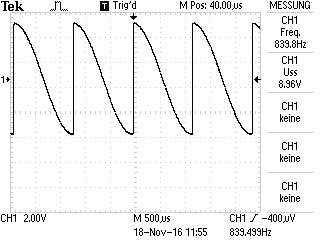
\includegraphics[width=\textwidth]{Bilder/15.jpg}
\label{fig:1}
\caption{$\varphi = 15\si{\degree}$}
\end{minipage}
\hspace{10pt}
\vspace{5pt}
\begin{minipage}[t]{0.3\textwidth}
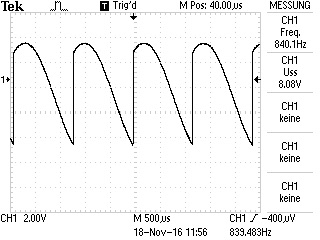
\includegraphics[width=\textwidth]{Bilder/45.jpg}
\label{fig:2}
\caption{$\varphi = 45\si{\degree}$}
\end{minipage}
\hspace{10pt}
\vspace{5pt}
\begin{minipage}[t]{0.3\textwidth}
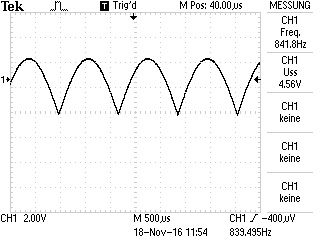
\includegraphics[width=\textwidth]{Bilder/105.jpg}
\label{fig:3}
\caption{$\varphi = 105\si{\degree}$}
\end{minipage}
\hspace{10pt}
\vspace{5pt}
\begin{minipage}[t]{0.3\textwidth}
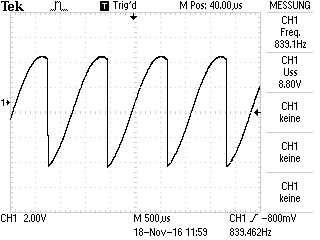
\includegraphics[width=\textwidth]{Bilder/165.jpg}
\label{fig:4}
\caption{$\varphi = 165\si{\degree}$}
\end{minipage}
\hspace{12pt}
\vspace{5pt}
\begin{minipage}[t]{0.3\textwidth}
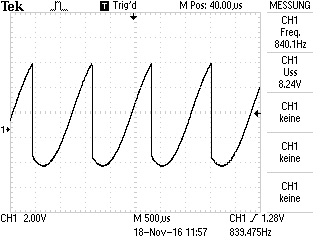
\includegraphics[width=\textwidth]{Bilder/225.jpg}
\label{fig:5}
\caption{$\varphi = 225\si{\degree}$}
\end{minipage}
\hspace{12pt}
\vspace{5pt}
\begin{minipage}[t]{0.3\textwidth}
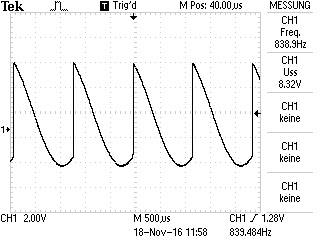
\includegraphics[width=\textwidth]{Bilder/330.jpg}
\label{fig:6}
\caption{$\varphi = 330\si{\degree}$}
\end{minipage}
\hspace{12pt}
\vspace{5pt}
\end{figure}

% \begin{itemize}
%   \item Abbildung \ref{fig:1}: Annäherung des Signals durch eine Fourierreihe.
%   \item Abbildung \ref{fig:2}: Übergang durch Phasenänderung um 45\si{\degree}.
%   \item Abbildung \ref{fig:3}: Weitere Phasenänderung um 45\si{\degree}, symmetrisch zur x-Achse.
%   \item Abbildung \ref{fig:4}: Fast vollständige Umkehrung, ingesamt um 135\si{\degree} gedreht.
%   \item Abbildung \ref{fig:5}: Komplette Drehung um 180\si{\degree}, gespiegelt an der $x$-Achse zum Ausgangssignal.
% \end{itemize}

Oben zu sehen sind die Aufzeichnungen des Oszilloskopes ohne den Tiefpassfilter.
\newpage

\begin{figure}[!h]
\begin{minipage}[t]{0.3\textwidth}
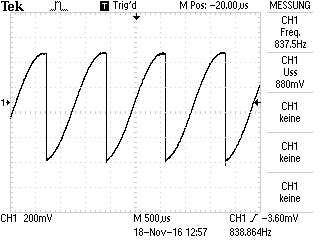
\includegraphics[width=\textwidth]{Bilder/Rausch0.jpg}
\label{fig:}
\caption*{$\varphi = 0\si{\degree}$}
\end{minipage}
\hspace{10pt}
\vspace{5pt}
\begin{minipage}[t]{0.3\textwidth}
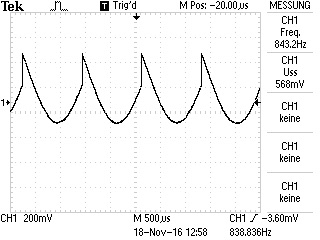
\includegraphics[width=\textwidth]{Bilder/Rausch120.jpg}
\label{fig:8}
\caption*{$\varphi = 45\si{\degree}$}
\end{minipage}
\hspace{10pt}
\vspace{5pt}
\begin{minipage}[t]{0.3\textwidth}
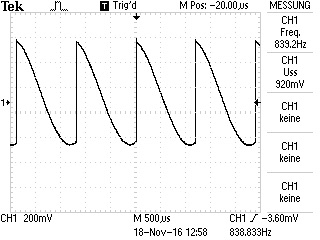
\includegraphics[width=\textwidth]{Bilder/Rausch165.jpg}
\label{fig:9}
\caption*{$\varphi = 90\si{\degree}$}
\end{minipage}
\hspace{10pt}
\vspace{5pt}
\begin{minipage}[t]{0.3\textwidth}
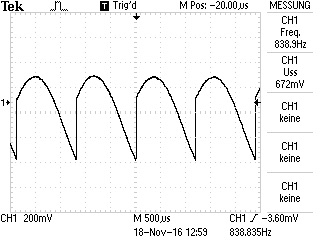
\includegraphics[width=\textwidth]{Bilder/Rausch240.jpg}
\label{fig:10}
\caption*{$\varphi = 135\si{\degree}$}
\end{minipage}
\hspace{12pt}
\vspace{5pt}
\begin{minipage}[t]{0.3\textwidth}
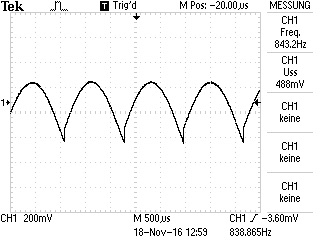
\includegraphics[width=\textwidth]{Bilder/Rausch270.jpg}
\label{fig:11}
\caption*{$\varphi = 180\si{\degree}$}
\end{minipage}
\hspace{12pt}
\vspace{5pt}
\begin{minipage}[t]{0.3\textwidth}
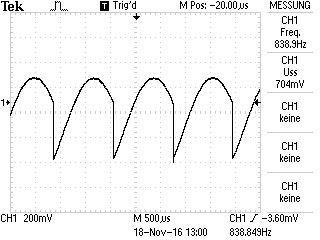
\includegraphics[width=\textwidth]{Bilder/Rausch315.jpg}
\label{fig:12}
\caption*{$\varphi = 180\si{\degree}$}
\end{minipage}
\hspace{12pt}
\vspace{5pt}
\end{figure}

% Für die Messwerte mit Rauschen und ohne Tiefpassfilter folgt die analoge Beschreibung der Grafiken. Anzumerken ist hier,
% dass sich die Graphen gespiegelt zur $x$-Achse verhalten. \\
%
% Im nächsten Auswertungsteil geht es um die Abhängigkeit der Ausgangsspannung zur Phasenverschiebung.
% Dazu wird zunächst das nicht verrauschte Signal verwendet. Die Messdaten zu der Versuchsreihe sind Tabelle \ref{tab:oRmT}
% zu entnehmen. Die Phasendifferenz wird für eine bessere Darstellung gegen die Ausgangsspannung U$_\text{out}$ geplottet.
% \begin{figure}[!h]
%   \centering
%   \includegraphics[width=1.0\textwidth]{Plots/Plot_Messung_oR.pdf}
%   \caption{Ausgangsspannung U$_\text{out}$ in Abhängigkeit von der Phasendifferenz $\Delta\varphi$.}
%   \label{fig:Uout}
% \end{figure}
